\newgeometry{left=1cm, right=1cm, bottom=2cm}

\begin{figure}
	\centering
	\begin{subfigure}{0.375\textwidth}
		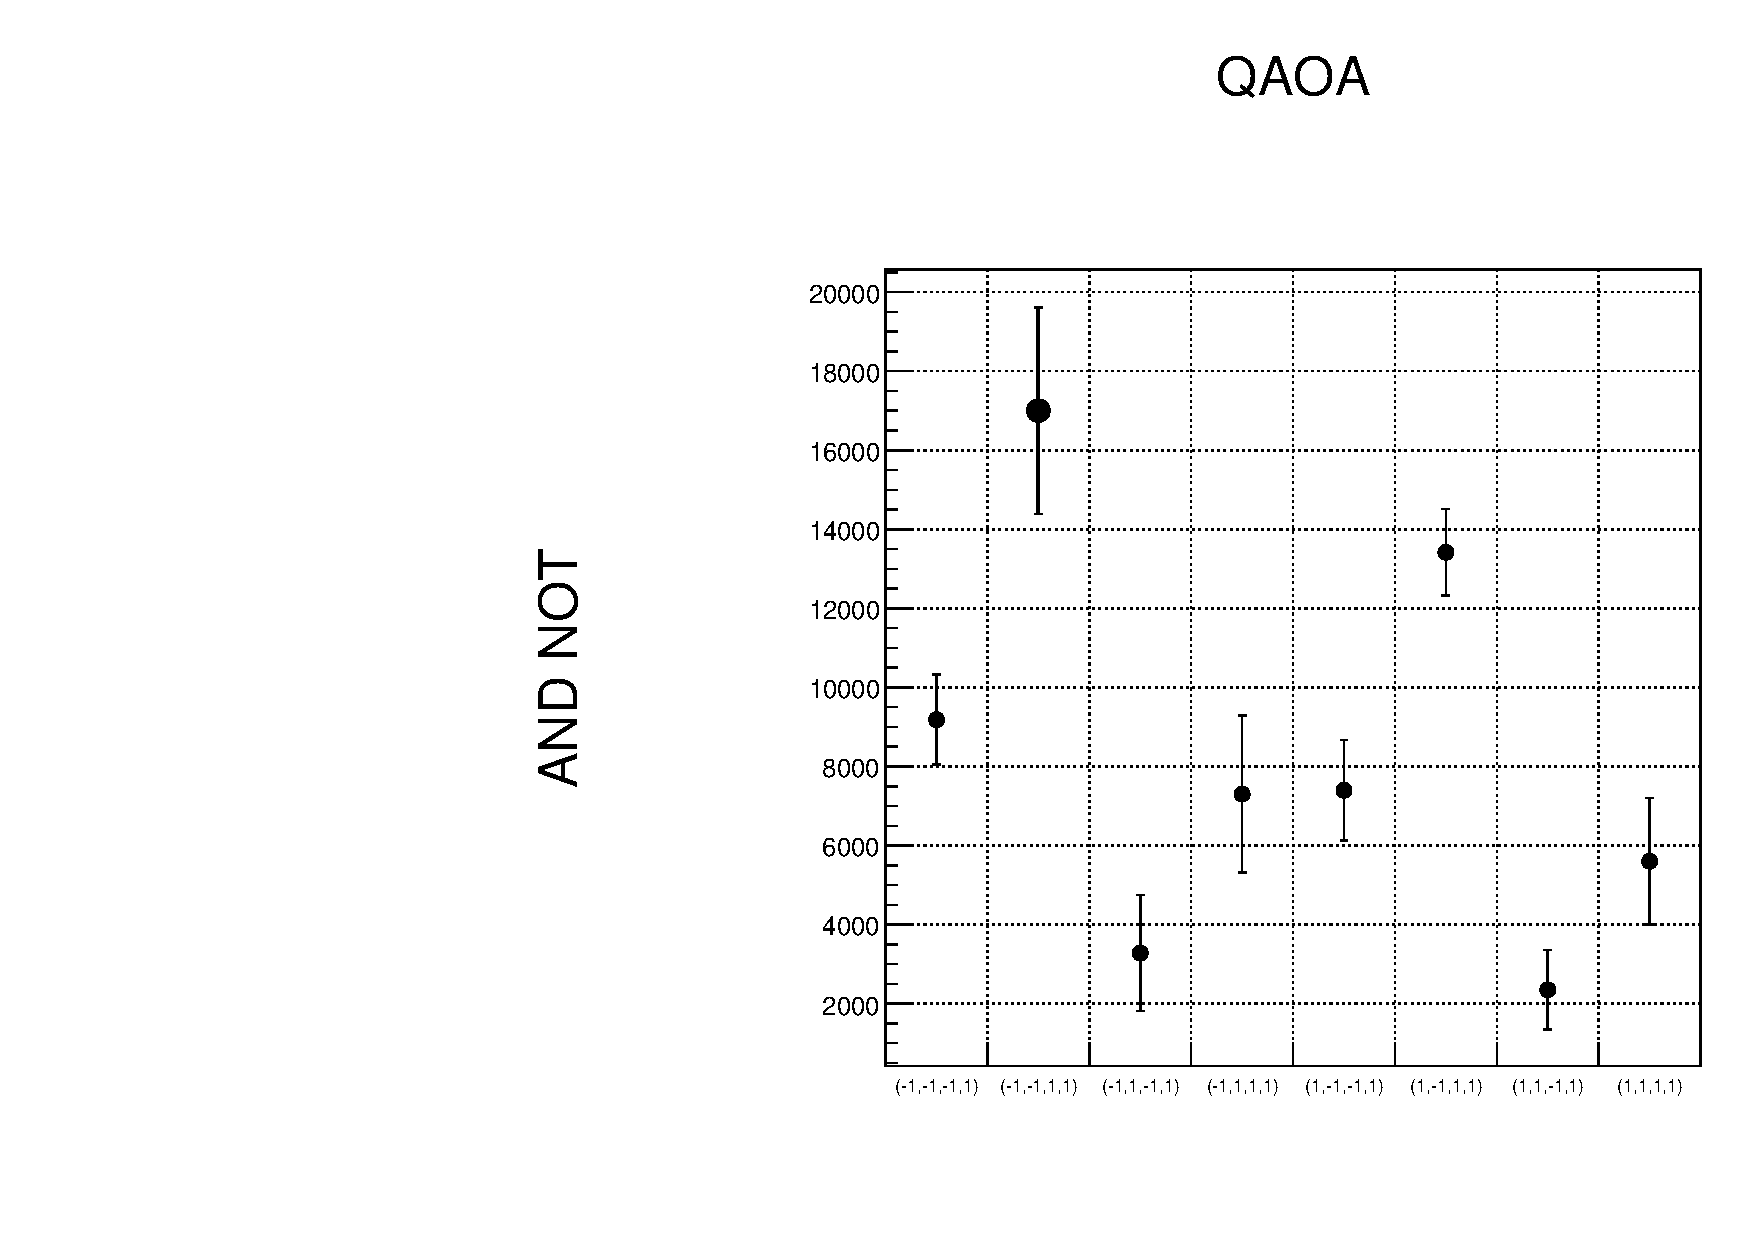
\includegraphics[width=\textwidth]{Pictures/0}
	\end{subfigure}
	\hspace{-1.5cm}
	\begin{subfigure}{0.375\textwidth}
		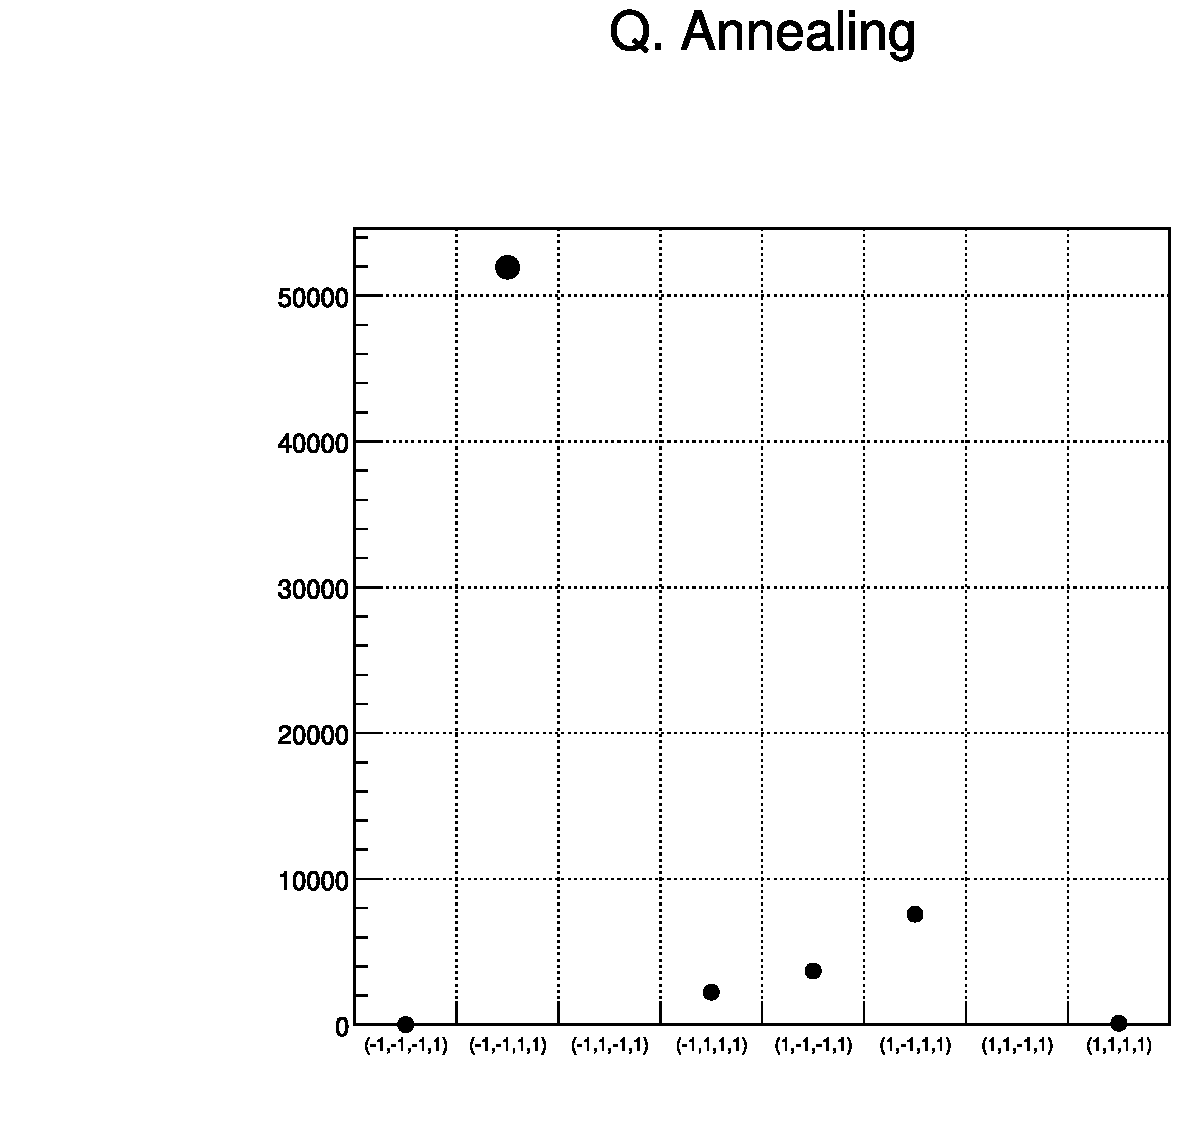
\includegraphics[width=\textwidth]{Pictures/1}
	\end{subfigure}
	\hspace{-1.5cm}
	\begin{subfigure}{0.375\textwidth}
		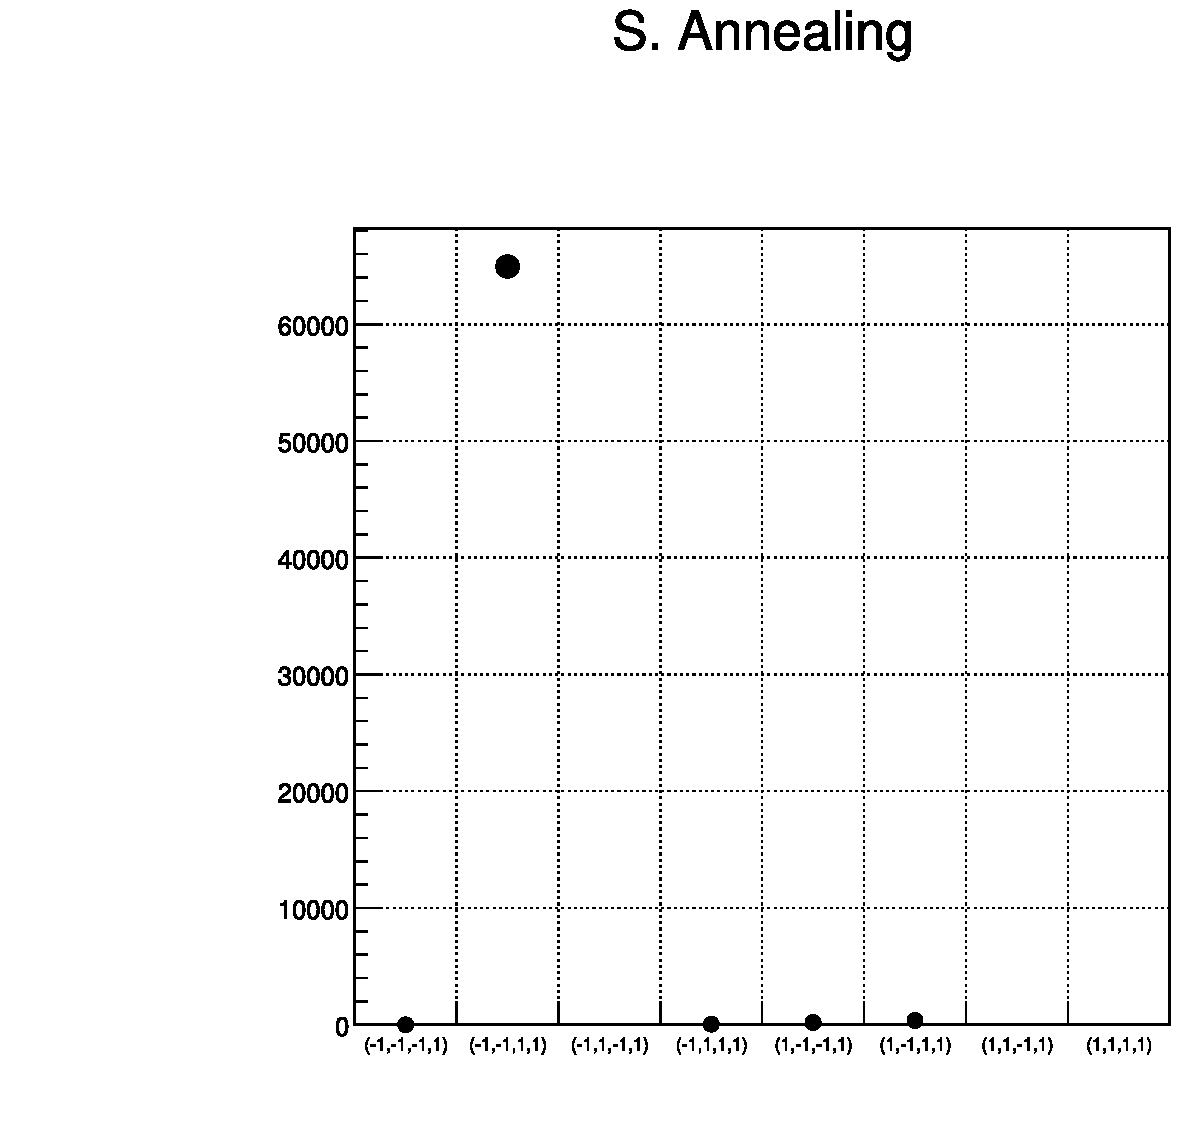
\includegraphics[width=\textwidth]{Pictures/2}
	\end{subfigure}
	
	\vspace{-1.5cm}
	
	\begin{subfigure}{0.375\textwidth}
		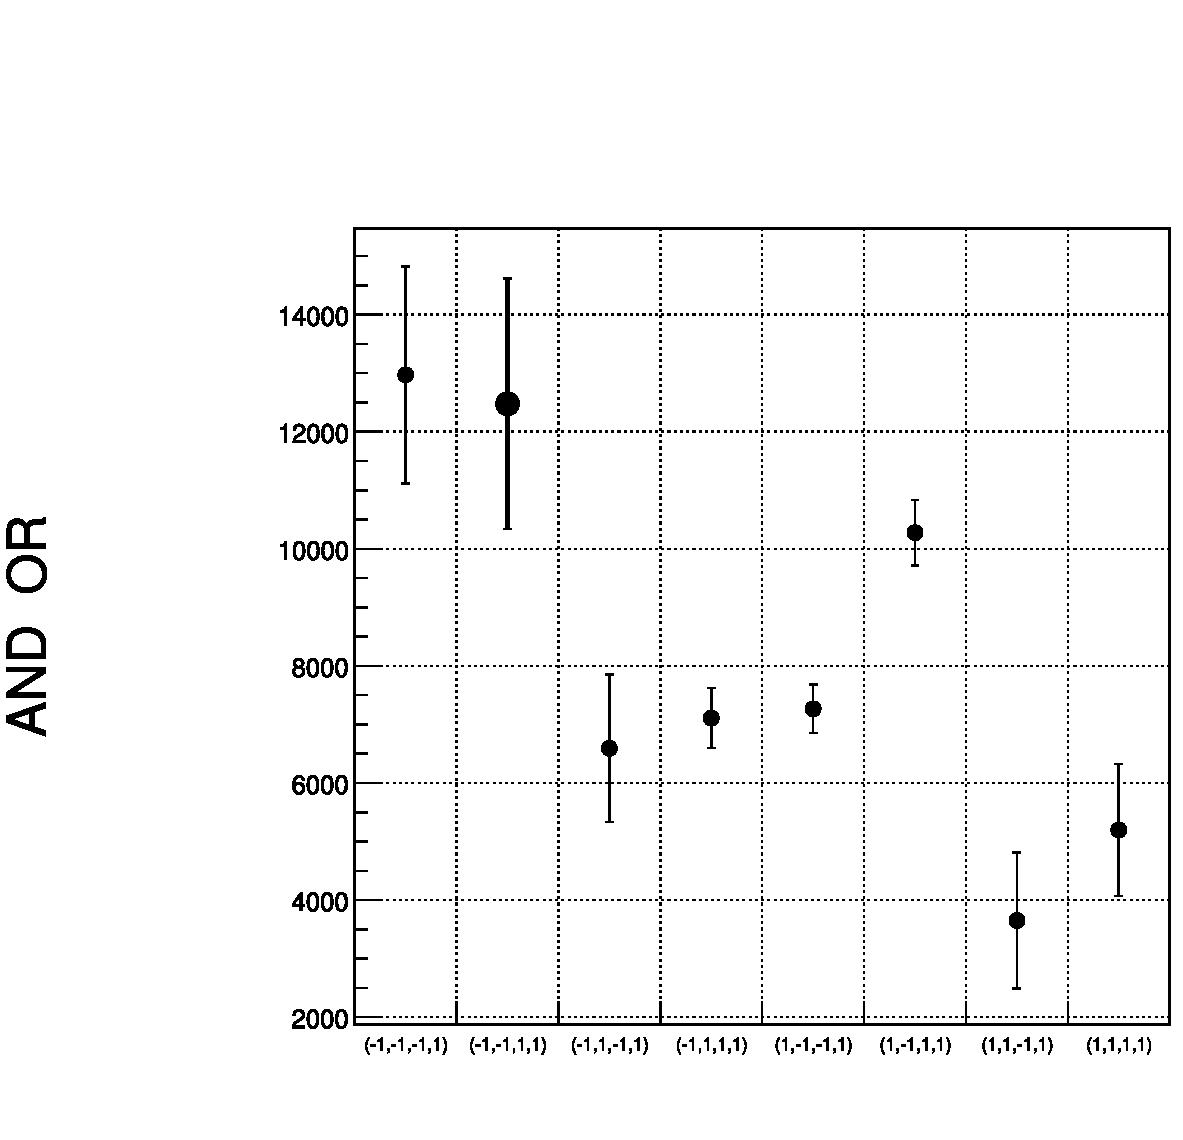
\includegraphics[width=\textwidth]{Pictures/3}
	\end{subfigure}
	\hspace{-1.5cm}
	\begin{subfigure}{0.375\textwidth}
		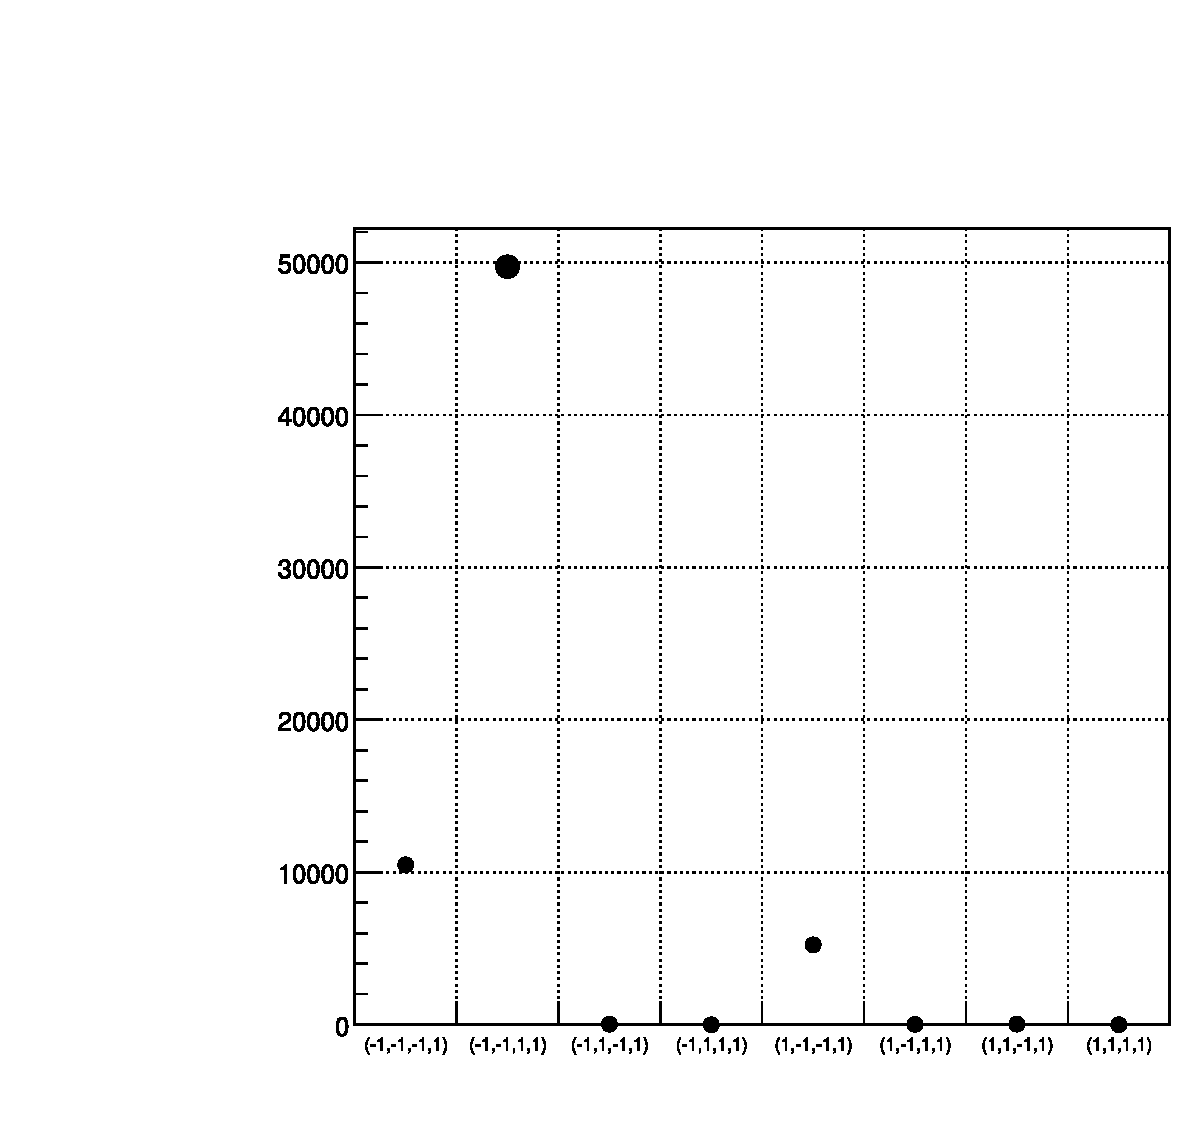
\includegraphics[width=\textwidth]{Pictures/4}
	\end{subfigure}
	\hspace{-1.5cm}
	\begin{subfigure}{0.375\textwidth}
		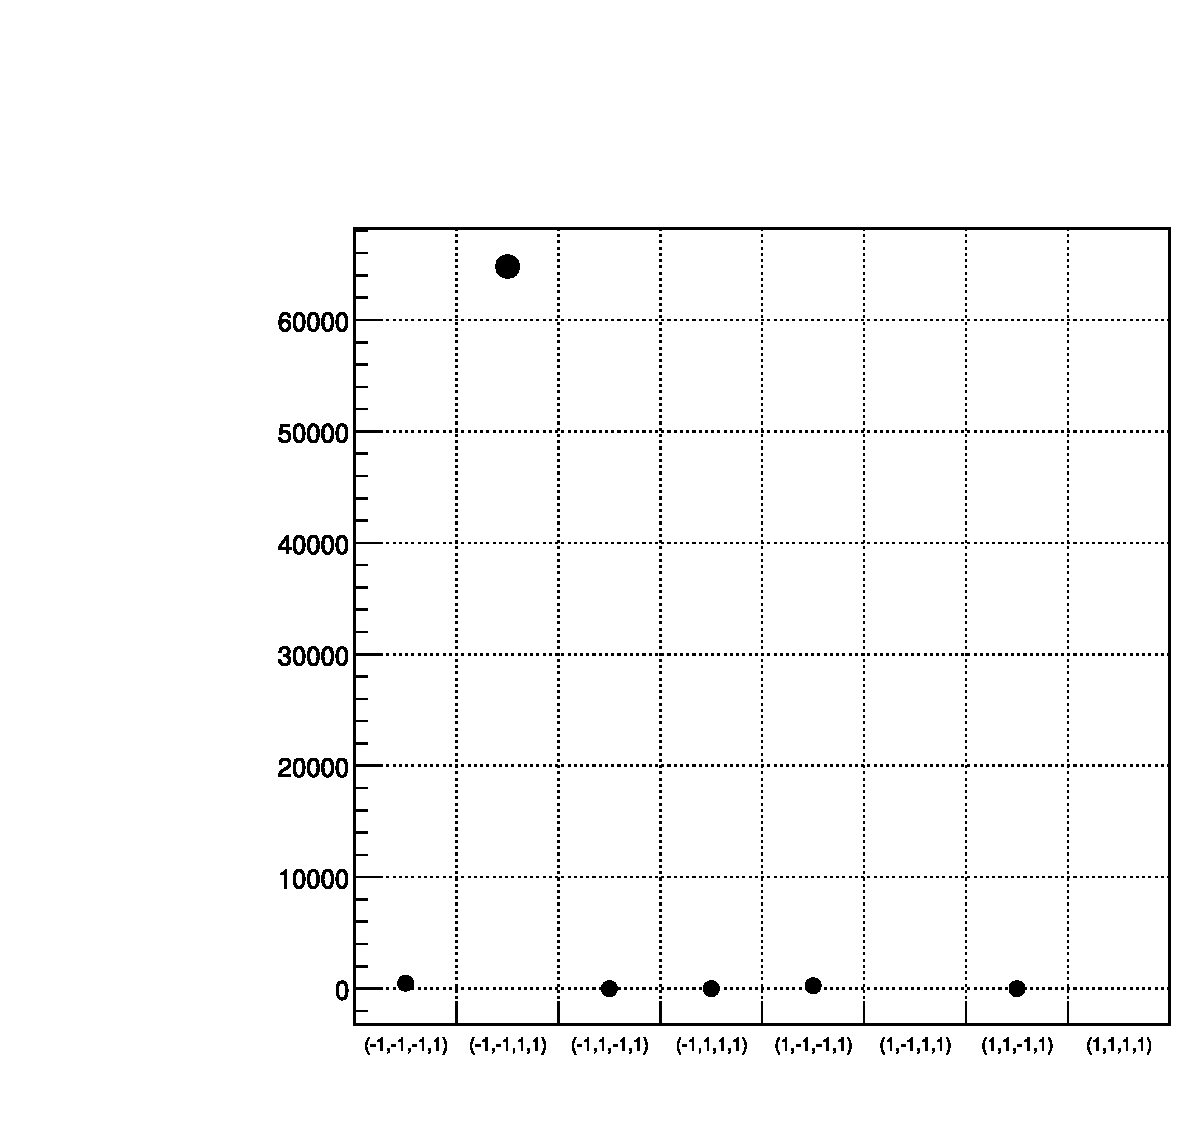
\includegraphics[width=\textwidth]{Pictures/5}
	\end{subfigure}
	
	\vspace{-1.5cm}
	
	\begin{subfigure}{0.375\textwidth}
		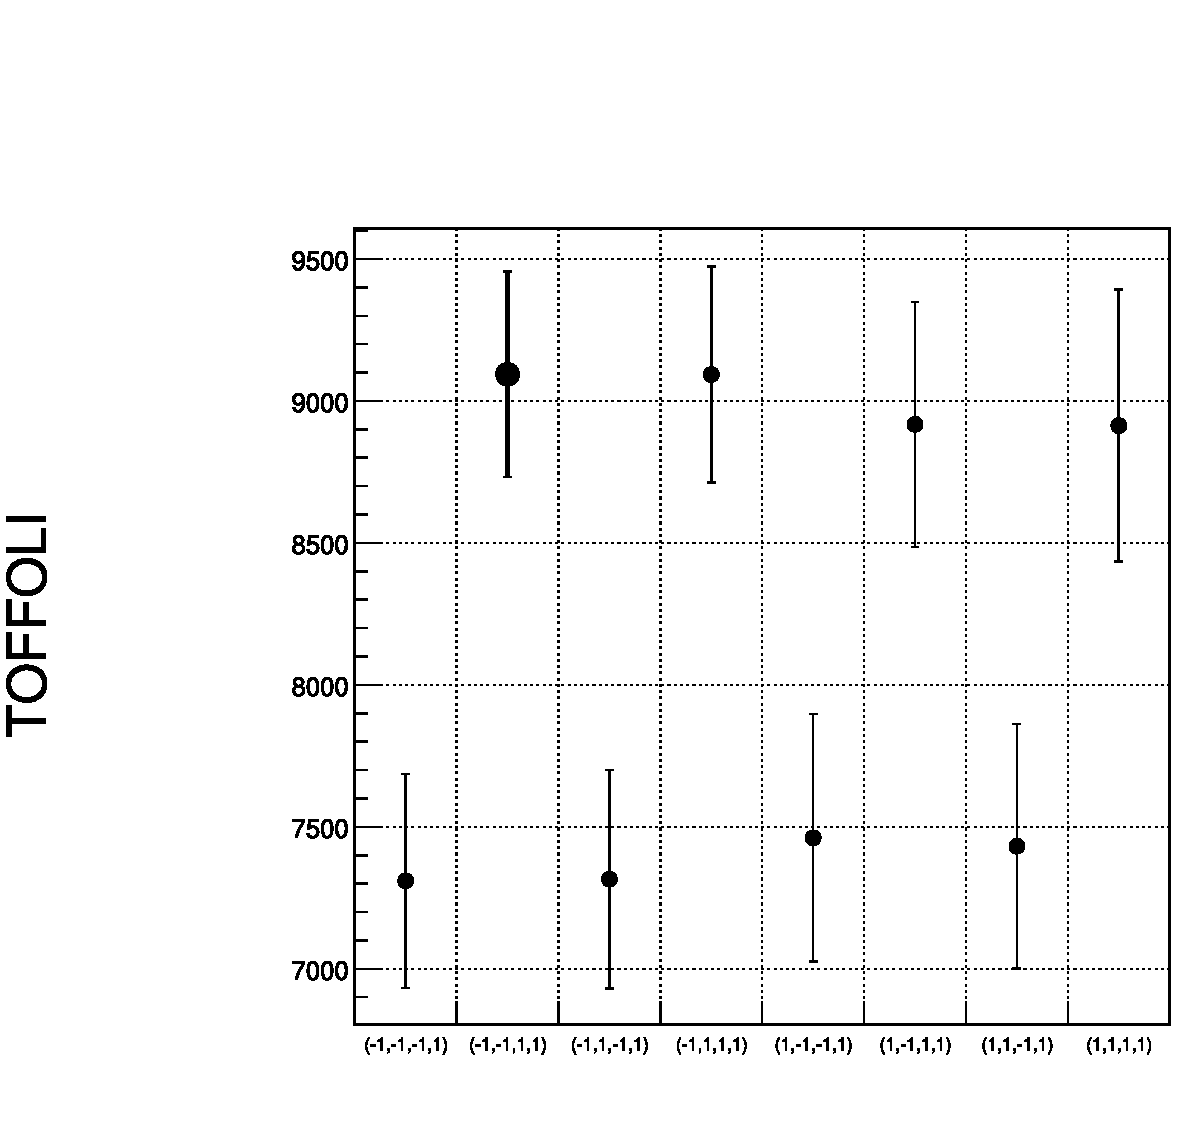
\includegraphics[width=\textwidth]{Pictures/6}
	\end{subfigure}
	\hspace{-1.5cm}
	\begin{subfigure}{0.375\textwidth}
		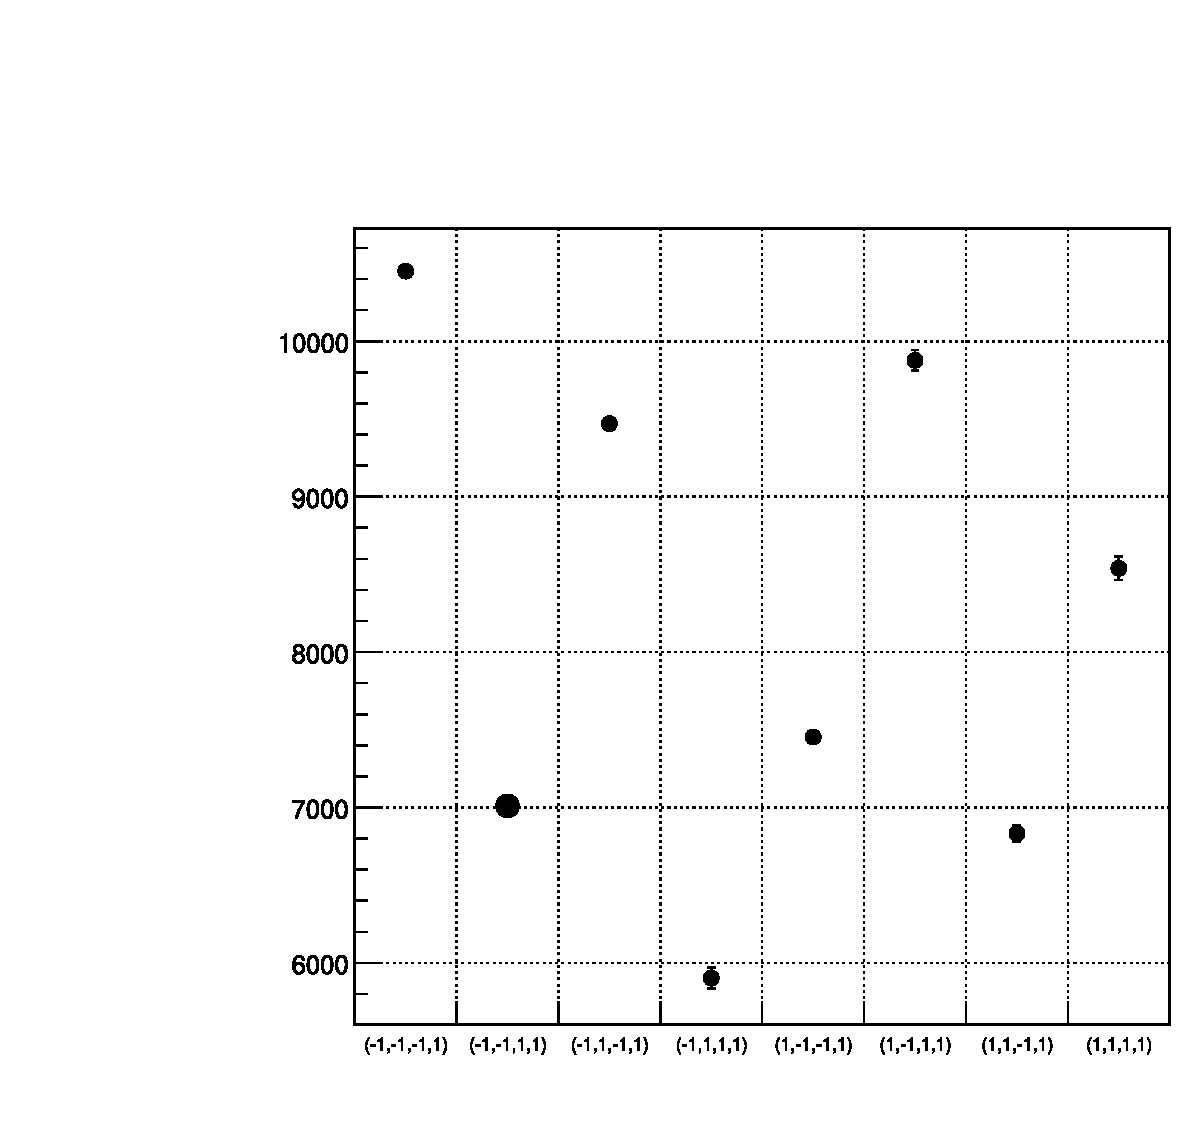
\includegraphics[width=\textwidth]{Pictures/7}
	\end{subfigure}
	\hspace{-1.5cm}
	\begin{subfigure}{0.375\textwidth}
		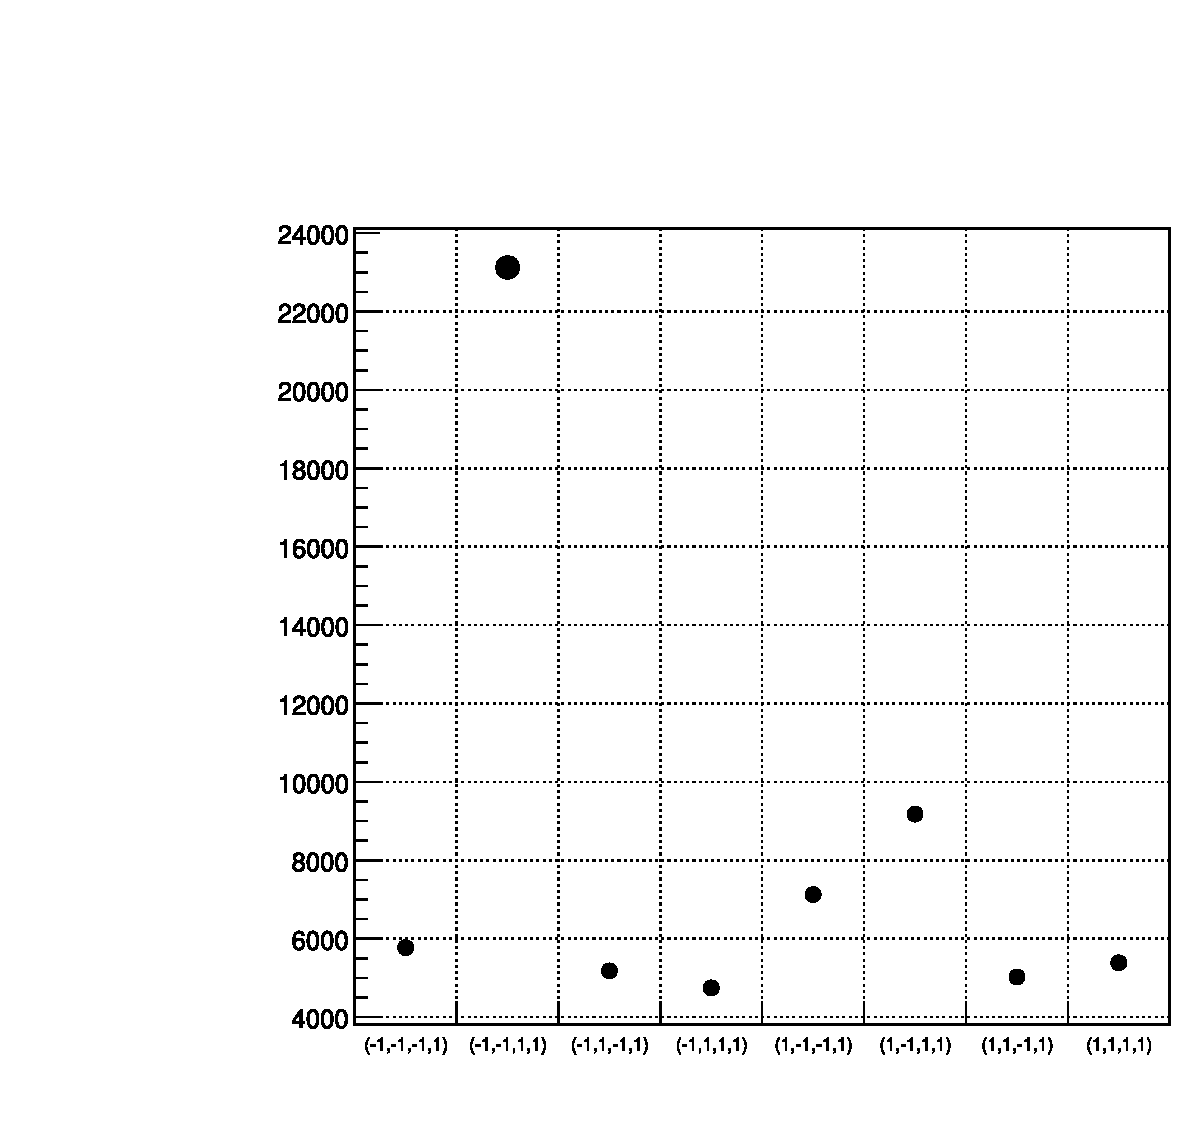
\includegraphics[width=\textwidth]{Pictures/8}
	\end{subfigure}
	
	\vspace{-1.5cm}
	
	\begin{subfigure}{0.375\textwidth}
		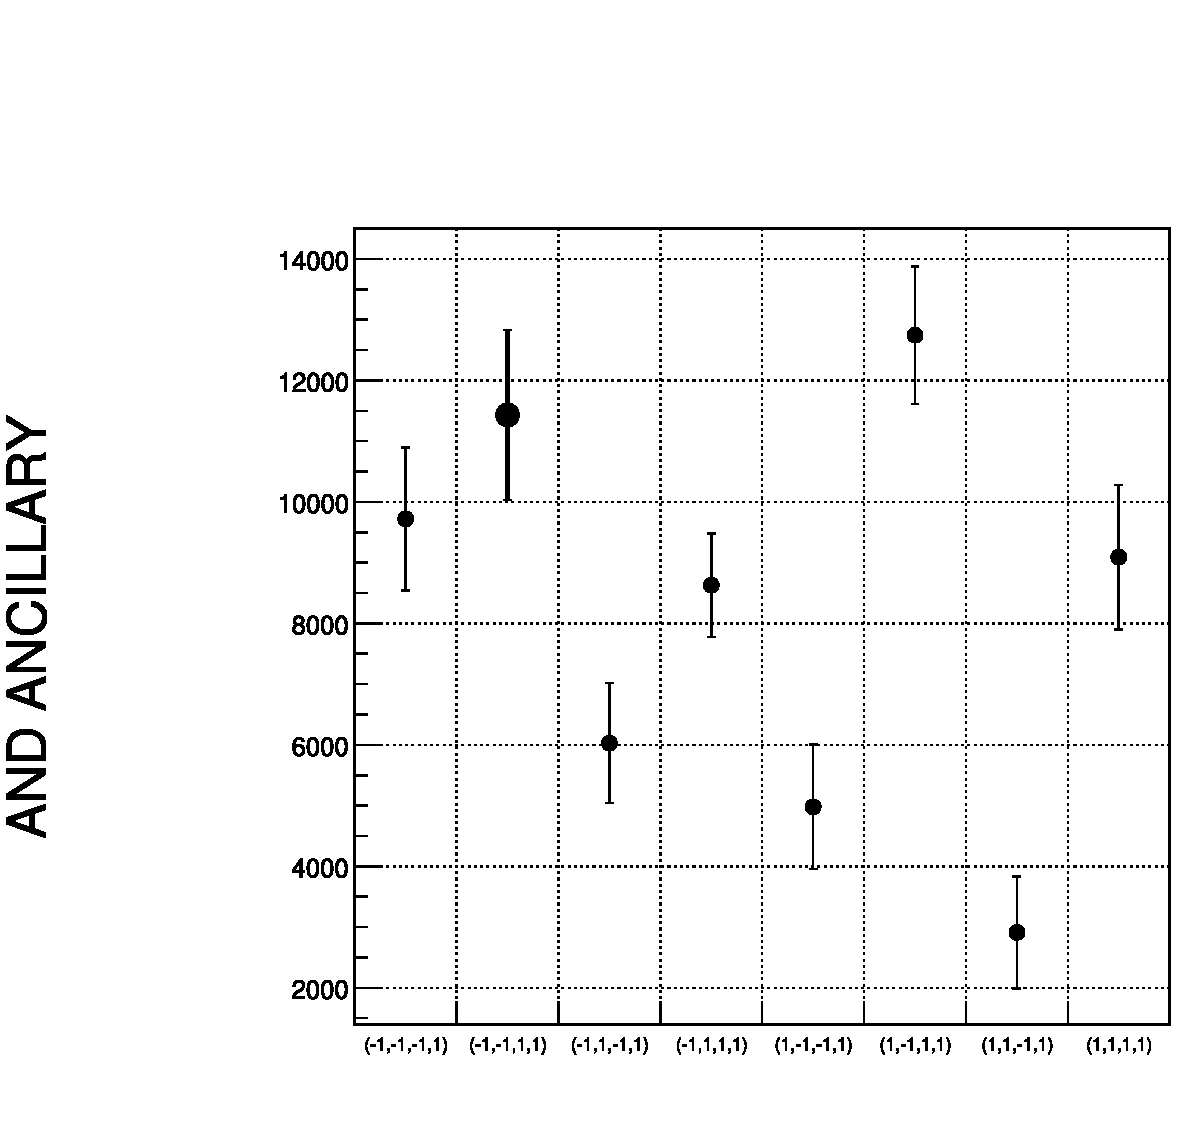
\includegraphics[width=\textwidth]{Pictures/9}
	\end{subfigure}
	\hspace{-1.5cm}
	\begin{subfigure}{0.375\textwidth}
		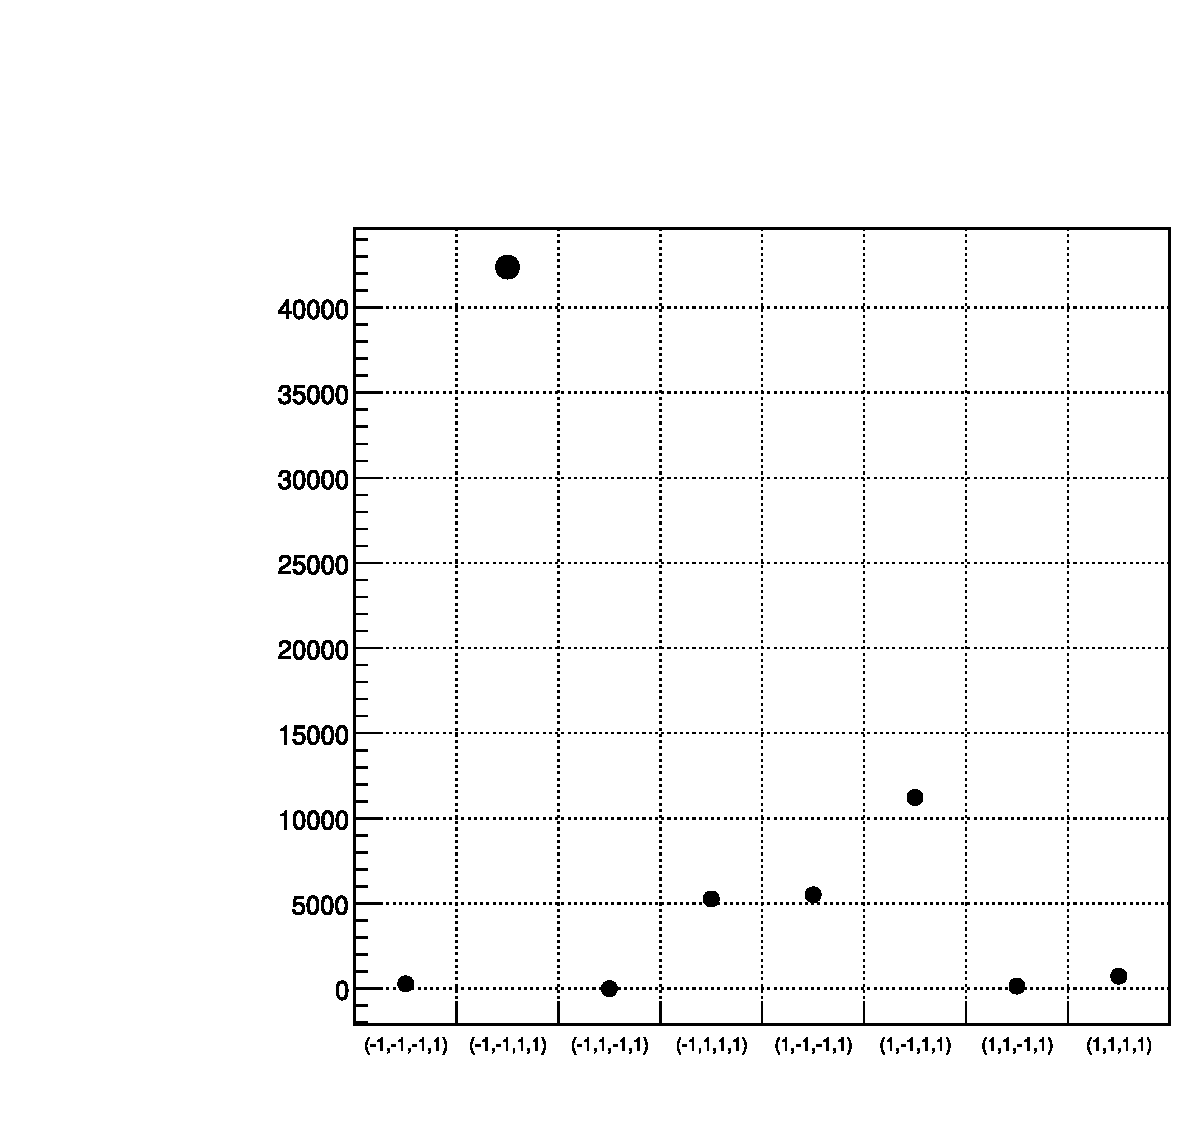
\includegraphics[width=\textwidth]{Pictures/10}
	\end{subfigure}
	\hspace{-1.5cm}
	\begin{subfigure}{0.375\textwidth}
		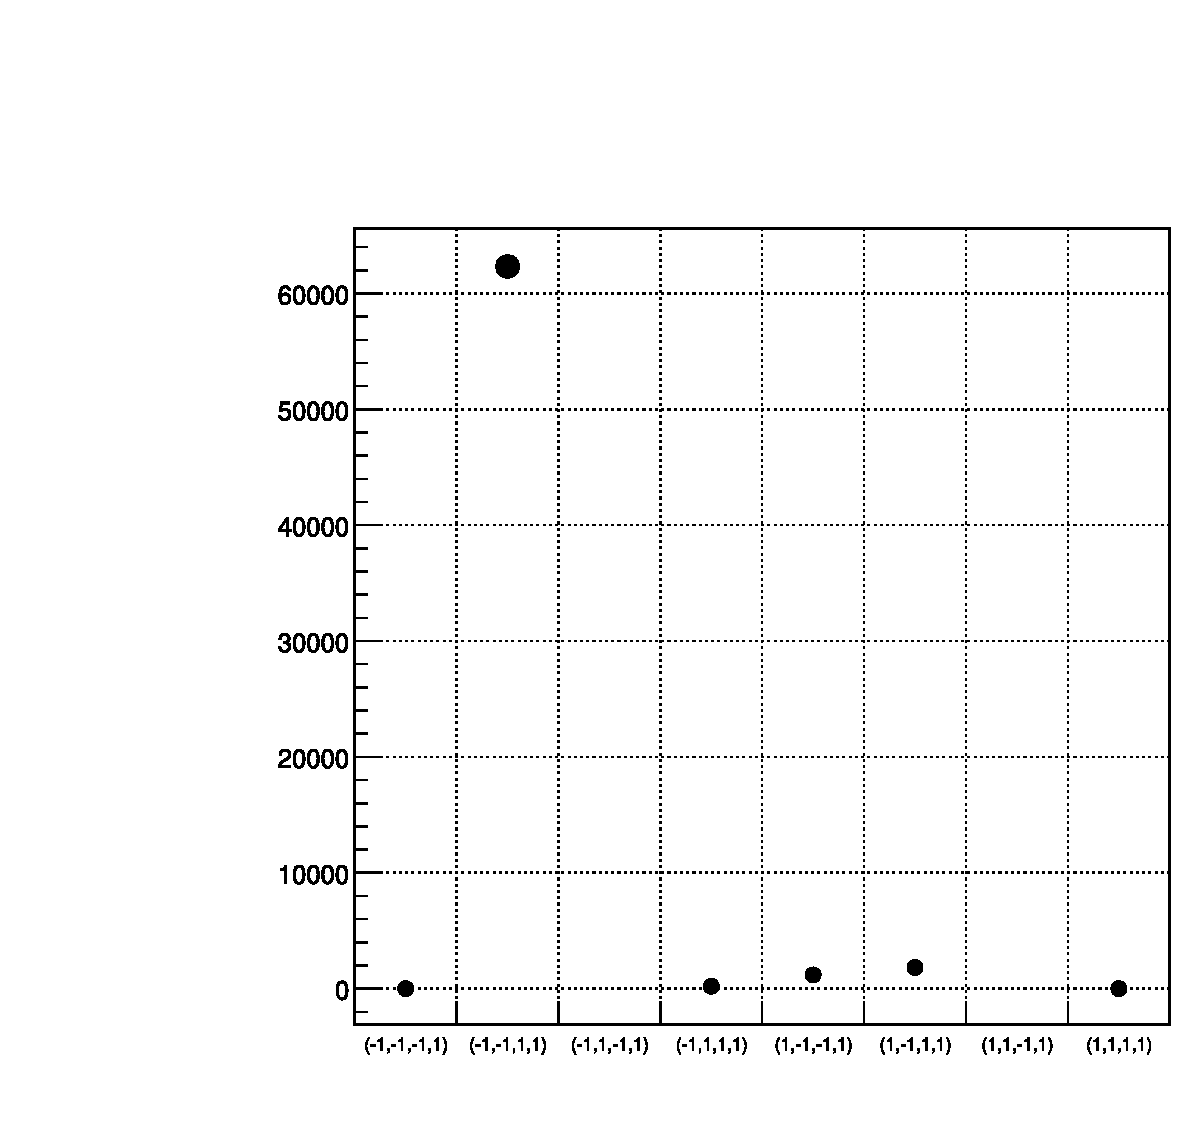
\includegraphics[width=\textwidth]{Pictures/11}
	\end{subfigure}
	
	\caption{Risultati}
	\label{fig:results}
\end{figure}
\restoregeometry